\subsection*{Fundamental Particles of the Standard Model}
\begin{tabular}{|| c| p{3cm}| *{4}{c|}  |}
\hline\hline
 symbol & name & type &  $J^{PC}$ & Q & mass\\
        &      &      &           &   &      
\\\hline
 $\gamma$ & photon & gauge boson & $1^{--}$ & $0$ & 0
\\\hline
 $g$ & gluon & gauge boson & $1^{--}$ & $0$ & 0 
\\\hline
 $W^+$ & W & gauge boson & $1$ & $+1$ & 80 GeV 
\\\hline
 $Z$ & Z & gauge boson & $1$ & $0$ & 91 GeV
\\\hline\hline
$H$ & Higgs & boson & $0^{++}$ & $0$ & 125 GeV
\\\hline\hline
\end{tabular}

\begin{tabular}{|| c| p{3cm}| *{4}{c|} |}
\hline\hline
 symbol & name & type &  $J^{P}$ & Q & mass \\
        &      &      &          &   &      
\\\hline
 $e^-$   & electron, ``e-minus'' & lepton & \half & $-1$ & 0.511 MeV
\\\hline
 $\nu_{e}$   & electron neutrino, ``nu-e''& lepton & \half & $0$ & tiny
\\\hline
 $\mu^-$   & muon, ``mu'', ``mu-minus'' & lepton & \half & $-$1 & 106 MeV
\\\hline
 $\nu_{\mu}$   & muon neutrino, ``nu-mu''& lepton & \half & $0$ & tiny
\\\hline
 $\tau^-$   & tau, tau-minus& lepton & \half & $-1$ & 1.78 GeV
\\\hline
 $\nu_{\tau}$   & tau neutrino, ``nu-tau''& lepton & \half & $0$ & tiny
\\\hline\hline
\end{tabular}

\begin{tabular}{|| c| p{3cm}| *{4}{c|} |}
\hline\hline
 symbol & name & type &  $J^{P}$ & Q & mass \\
        &      &      &          &   &      
\\\hline
 u     & up & quark & $\half^+$ & $+2/3$ & 1.5-3 MeV
\\\hline
 d     & down & quark & $\half^+$ &$ -1/3$ & 3-7 MeV
\\\hline
 c     & charm & quark & $\half^+$ & $+2/3$ & 1.3 GeV
\\\hline
 s     & strange & quark & $\half^+$ & $-1/3$ & $\sim 100$ MeV
\\\hline
 t     & top (truth)& quark & $\half^+$ & $+2/3$ & 173 GeV
\\\hline
 b     & bottom (beauty) & quark & $\half^+$ & $-1/3$ & 4.2 GeV
\\\hline\hline
\end{tabular}
\\

\paragraph{Parity (P) eigenvalue of a two body system}
If each particle is a P eigenstate:
\[
P = (-1)^{L} \times \prod\limits_{\mathsf{all\;particles}} \mbox{(intrinsic parity)}
\]
where L is the angular momentum quantum number for this 2-particle system.

The intrinsic parity of a fermion-antifermion pair is $-1$, so, for
pair of spin-\half\ fermions $ P =(-1)^{L+1}$.

\paragraph{C- eigenvalue of multibody system}
For a system of $C$-eigenstates:
\[
\prod\limits_{\mathsf{all\;particles}}
\mbox{(intrinsic C)}
\]
For a particle anti-particle pair of bosons that are not $C$
eigenstates (e.g. $\pi^+\pi^-$):
\[
C = (-1)^L
\]
For a fermion-antifermion pair (e.g. $e^+ e^-$) with relative angular
momentum $L$ and and total spin $S$:
\[
C = (-1)^{L+S}
\]


\subsection*{CKM matrix}

\begin{equation}
\label{eq:th.b.ckmlabel}
  V_{\mathrm{CKM}}=\mIII{ V_{ud} }{ V_{us} }{ V_{ub} }{
                        V_{cd} }{ V_{cs} }{ V_{cb} }{
                        V_{td} }{ V_{ts} }{ V_{tb} }
\approx
                 \mIII{ 0.974 }{ 0.225 }{ 0.00371\cdot e^{-i \gamma} }{
                        -0.225 }{ 0.973}{0.0418 }{
                        0.00868\cdot e^{-i \beta} }{-0.0411 }{0.99912 }
\end{equation}
where $\gamma \approx 68^o$ and $\beta = 21^o$.

\subsection*{\emph{The} Unitarity triangle}
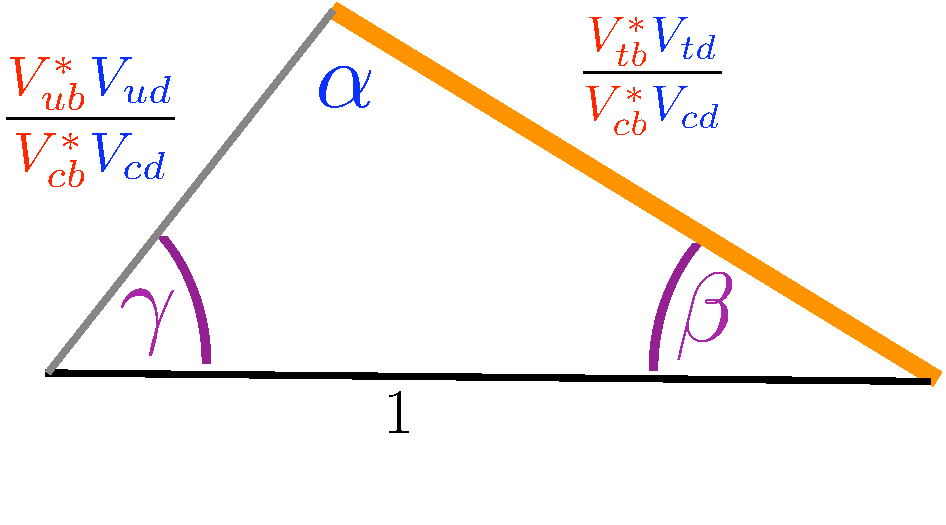
\includegraphics[width=0.5\textwidth]{fig/UT}

\subsection*{Meson, Baryon properties}

\newcommand{\fste}[1]{
{\raggedright
#1
}}
\newcommand{\ioa}{
\fste{its own antiparticle}
}

\newcommand{\tabletitle}[1]{
\paragraph{#1}\mbox{}\\
}
\tabletitle{Light ``unflavoured'' mesons:}
\begin{tabular}{|| c| l| *{7}{c|} p{2.3cm} ||}
\hline\hline
 symbol & name & type &  I & $I_3$ & $J^{PC}$ & Q & mass & quark & comment\\
        &      &      &    &&       &   &      & cont. &  
\\\hline\hline
 $\pi^{+}$     & pion & meson & 1 & $+1$ & $0^{-}$ & $+1$ & 140 MeV &
 $u\overline{d}$ 
&''stable''\footnotemark[1]
\\\hline
 $\pi^{-}$     & pion & meson & 1 & $-1$ & $0^{-}$ & $-1$ & 140 MeV &
 $\overline{u}d$
&''stable''\footnotemark[1]
\\\hline
 $\pi^0$    & pion & meson & 1 & $0$ & $0^{-+}$ & 0 & 135 MeV &
 $\frac{u\overline{u} - d\overline{d}}{\sqrt{2}}$ & \ioa
%, decays
% to $\gamma\gamma$
\\\hline
 $\eta$    & eta & meson & 0 & $0$ & $0^{-+}$ & 0 & 545 MeV &
 $\frac{u\overline{u} + d\overline{d} - 2s\overline{s}}{\sqrt{6}}$ & \ioa
\\\hline
 $\eta'$    & eta-prime & meson & 0 & $0$ & $0^{-+}$ & 0 & 958 MeV &
 $\frac{u\overline{u} + d\overline{d} + s\overline{s}}{\sqrt{3}}$ & \ioa
\\\hline
\end{tabular}

\tabletitle{More ``unflavoured'' mesons:}
\begin{tabular}{|| c| l| *{6}{c|} p{1.2cm} | p{2.3cm} ||}
\hline\hline
 symbol & name & type &  I & $I_3$ & $J^{PC}$ & Q & mass & quark & comment\\
        &      &      &    &&       &   &      & cont. & 
\\\hline\hline
 $\rho^+(770)$    & rho & meson  & 1 & $+1$ & $1^{-}$ & $+1$ & 776 MeV &
$u\overline{d}$ &
 %decays to $\pi^+\pi^0$
\\\hline
 $\rho^0(770)$    & rho & meson  & 1 & $0$ & $1^{--}$ & 0 & 776 MeV &
 $u\overline{u}, d\overline{d}$  & \ioa 
%Decays
% mainly to $\pi^+ \pi^-$
\\\hline
 $\omega(782)$    & omega & meson & 0 & 0 & $1^{--}$ & 0 & 783 MeV &
 $u\overline{u}, d\overline{d}$  & \ioa 
%Decays
% mainly to $\pi^+ \pi^- \pi^0$
\\\hline
 $f_0(980)$    & f-zero & meson & 0 & 0 & $0^{++}$ & 0 & 990 MeV &
 $u\overline{u}$, $d\overline{d}$, $s\overline{s}$ 
 & \ioa
% Decays
% mainly to $\pi\pi$
\\\hline
 $\phi$    & phi & meson & 0 & 0 & $1^{--}$ & 0 & 1.02 GeV &
 $s\overline{s}$ & \ioa
%\\\multicolumn{10}{||c||}{\parbox{0.9\textwidth}{
%\ioa, decays mainly to $K^+K^-$ (49\%) $K_L^0
% K_S^0$ (34\%)}}
\\\hline
\end{tabular}

\tabletitle{Strange mesons:}
For the following mesons you can deduce isospin and $I_3$ from the quark
content. $u, d$ have $I=\half$ and $I_3 = +\half, -\half$
respectively. All other quarks have $I=0$.
\\
\begin{tabular}{|| c| p{1.5cm}| *{5}{c|} p{2.7cm} ||}
\hline\hline
 symbol & name & type &  $J^{PC}$ & Q & mass & quark & comment\\
        &      &      &           &   &    & cont. & 
\\\hline
 $K^+$    & Kaon & meson & $0^{-}$ & +1 & 494 MeV &
 $u\overline{s}$ & ``stable'' \footnotemark[1]
\\\hline
 $K^0$    & Kaon & meson & $0^{-}$ & 0 & 498 MeV &
 $d\overline{s}$ & \fste{\emph{not} \ioa}
\\\hline
 $K_S$    & K-short & meson & $0^{-}$ & 0 & 498 MeV &
 $\approx \frac{d\overline{s} - s\overline{d}}{\sqrt{2}}$  & \\
\multicolumn{8}{||c||}{\parbox{0.9\textwidth}{
\emph{nearly} CP-even, $\tau = 0.09 ns$, tends to decay
 inside detector to $\pi\pi$ or $\pi^0\pi^0$.}}
\\\hline
 $K_L$    &K-long & meson & $0^{-}$ & 0 & 498 MeV &
  $\approx \frac{d\overline{s} + s\overline{d}}{\sqrt{2}}$  & \\
\multicolumn{8}{||c||}{\parbox{0.9\textwidth}{
\emph{nearly} CP-odd, $\tau = 51 \mathsf{ns}$, ``stable''\footnotemark[1]
}}
\\\hline
 $K^{*+}(892)$    & K-star & meson & $1^{-}$ & +1 & 892 MeV &
 $u\overline{s}$ & 
\\\hline
 $K^{*0}(892)$    & K-star & meson & $1^{-}$ & 0 & 892 MeV &
 $d\overline{s}$ & 
\\\hline\hline
\end{tabular}

\tabletitle{Heavy  mesons:}
\begin{tabular}{|| c| p{2cm}| *{5}{c|} p{2.4cm} ||}
\hline\hline
 symbol & name & type &  $J^{PC}$ & Q & mass & quark & comment\\
        &      &      &           &   &      & cont. &
\\\hline\hline
 $D^+$    & D, D-plus & meson & $0^{-}$ & +1 & 1.9 GeV &
 $c\overline{d}$ & \\
\multicolumn{8}{||c||}{\parbox{0.9\textwidth}{
unstable, lives long enough to travel short distances in detector ($\sim 1/3$ that
 of a B), many decay modes, often with Kaons}}
\\\hline
 $D^0$    & D, D-zero & meson & $0^{-}$ & 0 & 1.9 GeV &
 $c\overline{u}$ & \\
\multicolumn{8}{||c||}{\parbox{0.9\textwidth}{
\emph{not} its own antiparticle, unstable, lives long enough to travel short distances in detector ($\sim 1/3$ that
 of a B), many decay modes, often with Kaons}}
\\\hline
 $\overline{D}^0$    & D-bar, D-zero-bar & meson & $0^{-}$ & 0 & 1.9 GeV &
 $\overline{c}{u}$ & \fste{see comments for $D^0$}
\\\hline
 $D_s^+$    & D-sub-s & meson & $0^{-}$ & 0 & 2.0 GeV &
 $c\overline{s}$ &  \fste{see comments for $D^0$}
\\\hline
 $J/\psi$    & J-psi & meson & $1^{--}$ & 0 & 3.1 GeV &
 $c\overline{c}$ & 
\\\multicolumn{8}{||c||}{\parbox{0.9\textwidth}{
its own antiparticle, decays to particle-antiparticle pairs --- mainly
 hadrons. However, mostly reconstructed as $\mu^+\mu^-$ or $e^+ e^-$
 (BR $6\%$ each).}}
\\\hline
 $\Upsilon(4S)$    & Upsilon 4-S &  meson &$1^{--}$ & 0 & 10.6 GeV &
 $b\overline{b}$ & \fste{its own antiparticle, decays to \prt{B^0_d, \overline{B}^0_d} or \prt{B^+ B^-}}
\\\hline\hline
\end{tabular}

\footnotetext[1]{
 ``Stable'' means here that it won't decay within the time-scale it takes to traverse a
 detector like ATLAS, CMS, BaBar, LHCb etc.
}

\tabletitle{B-mesons:}
B mesons have a characteristically ``long'' lifetime ($\sim
1\,\mathsf{ps}$), resulting in sufficiently long flight distances that
their decay vertex can typically be distinguished from the production
vertex (if they are produced with sufficient boost, and the detector
resolution is good). They
have a large number of possible decay modes, often involving D mesons.\\
\begin{tabular}{|| c| p{2cm}| *{5}{c|} p{2.7cm} ||}
\hline\hline
 symbol & name & type &  $J^{PC}$ & Q & mass & quark & comment\\
        &      &      &           &   &      & cont. &
\\\hline\hline
 $B^+$    & B, B-u B-plus & meson & $0^{-}$ & +1 & 5.3 GeV &
 $\overline{b}u$ & 
\\\hline
 $B^0_d$    & B, B zero, B-sub-d & meson & $0^{-}$ & 0 & 5.3 GeV &
 $\overline{b}d$ &  also $B^0$
\\\hline
 $\overline{B}^0_d$    & B-bar, B zero-bar, anti-B & meson & $0^{-}$ & 0 & 5.3 GeV &
 ${b}\overline{d}$ & also $\overline{B}^0$
\\\hline
 $B^0_s$    & B-s, B-sub-s & meson & $0^{-}$ & 0 & 5.4 GeV &
 $\overline{b}s$ & 
\\\hline
 $\overline{B}^0_s$  & B-s-bar, B-sub-s-bar & meson & $0^{-}$ & 0 & 5.4 GeV &
 ${b}\overline{s}$ & 
\\\hline
 $B^{+}_c$    & B-c, B-sub-c & meson & $0^{-}$ & +1 & 6.3 GeV &
 $\overline{b}c$ & 
\\\hline
\end{tabular}

\tabletitle{A few baryons:}
\begin{tabular}{|| c| p{2.2cm}| *{6}{c|} p{1.2cm} ||}%% p{2.2cm} ||}
\hline\hline
 symbol & name & type &  $I$ & $I_3$ & $J^{PC}$ & Q & mass & quark\\  % & comment\\
        &      &      &      &  &      &   &      & cont.   %&
\\\hline\hline
$p$   & proton & baryon & \half & $+\half$ & $\half^+$ & $+1$ & 938.3 MeV &
$uud$ \\\hline
$n$   & neutron & baryon & \half & $-\half$ & $\half^+$ & $0$ & 939.6 MeV &
$udd$ \\\hline\hline
$\Lambda$ & Lambda & baryon & 0 & $0$ & $\half^+$ & 0 & 1.116 GeV & 
$uds$ \\\hline
$\Lambda_c$ & Lambda-c & baryon & 0 & $0$ & $\half^+$ & $+1$ & 2.286 GeV & 
$udc$ \\\hline
$\Lambda_b^0$    & Lambda-b & baryon &  0 & $0$ & $\half^+$ & 0 & 5.620 GeV &
 $udb$ \\\hline\hline
$\Sigma^+$ & Sigma & baryon & 1 & $+1$ & $\half^+$ &$+1$& 1.189 GeV &
$uus$
\\\hline
$\Sigma^0$ & Sigma & baryon & 1 & $0$ & $\half^+$ & $0$ & 1.193 GeV &
$uds$
\\\hline
$\Sigma^-$ & Sigma & baryon & 1 & $-1$ & $\half^+$ &$-1$& 1.197 GeV &
$dds$
\\\hline
$\Sigma^{++}_c$ & Sigma-c & baryon & 1 & $+1$ & $\half^+$ &$+2$& 2.454 GeV &
$uuc$
\\\hline
$\Sigma^+_c$ & Sigma-c & baryon & 1 & $0$ & $\half^+$ & $1$ & 2.453 GeV &
$udc$
\\\hline
$\Sigma^0_c$ & Sigma-c & baryon & 1 & $-1$ & $\half^+$ &$0$& 2.454 GeV &
$ddc$
\\\hline\hline
$\Xi^0$ & Xi/Cascade & baryon & \half & $+\half$ & $\half^+$ &$0$& 1.315 GeV &
$uss$
\\\hline
$\Xi^-$ & Xi/Cascade & baryon & \half & $-\half$ & $\half^+$ &$-1$& 1.321 GeV &
$dss$
\\\hline
$\Xi_c^+$ & Xi-c & baryon & \half & $+\half$ & $\half^+$ &$1$& 2.468 GeV &
$usc$
\\\hline
$\Xi_c^0$ & Xi-c & baryon & \half & $-\half$ & $\half^+$ &$0$& 2.471 GeV &
$dsc$
\\\hline\hline
$\Omega^-$ & Omega & baryon & 0 & $0$ & $\half^+$ & $-1$ & 1.672 GeV & 
$sss$ \\\hline
$\Omega_c^0$ & Omega-c & baryon & 0 & $0$ & $\half^+$ & $0$ & 2.698 GeV & 
$ssc$
\\\hline
$\Omega_b^0$ & Omega-b & baryon & 0 & $0$ & $\half^+$ & $0$ & 6.054 GeV & 
$ssb$
\\\hline\hline
\end{tabular}

\subsection*{Pauli matrices}
\[\sigma_{1}=\mII{0}{1}{1}{0},\sigma_{2}=\mII{0}{-i}{i}{0},\sigma_{3}=\mII{1}{0}{0}{-1}\]
%%
%%
